\documentclass[10pt]{article}
\usepackage{tikz}
\usepackage[margin=0cm]{geometry}
\pagestyle{empty}

\begin{document}

\vspace*{\fill}
\begin{center}
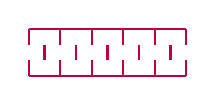
\begin{tikzpicture}[x=0.2cm, y=-0.2cm, thick, purple]
% North to South lines
    \draw (0,0) -- (0,1);
    \draw (0,2) -- (0,3);
    \draw (1,1) -- (1,2);
    \draw (2,0) -- (2,1);
    \draw (2,2) -- (2,3);
    \draw (3,1) -- (3,2);
    \draw (4,0) -- (4,1);
    \draw (4,2) -- (4,3);
    \draw (5,1) -- (5,2);
    \draw (6,0) -- (6,1);
    \draw (6,2) -- (6,3);
    \draw (7,1) -- (7,2);
    \draw (8,0) -- (8,1);
    \draw (8,2) -- (8,3);
    \draw (9,1) -- (9,2);
    \draw (10,0) -- (10,1);
    \draw (10,2) -- (10,3);
% North-West to South-East lines
% West to East lines
    \draw (0,0) -- (10,0);
    \draw (0,3) -- (10,3);
% South-West to North-East lines
\end{tikzpicture}
\end{center}
\vspace*{\fill}

\end{document}
